\documentclass[12pt,a4paper]{article}

% --- Page Layout -------------------------------------------------------------
\usepackage[a4paper, margin=0.8in, headheight=14pt]{geometry}

% --- Fonts (XeLaTeX) ---------------------------------------------------------
\usepackage{fontspec}
\usepackage{unicode-math}
\setmainfont{TeX Gyre Pagella}
\setmonofont[Scale=0.88]{TeX Gyre Cursor}
\setmathfont{Latin Modern Math}

% --- Packages ---------------------------------------------------------------
\usepackage{xcolor}
\usepackage{titlesec}
\usepackage{enumitem}
\usepackage{tabularx}
\usepackage{booktabs}
\usepackage{array}
\usepackage{amsmath}
\usepackage{tikz}
\usetikzlibrary{shapes.geometric, arrows.meta, positioning, calc, fit, decorations.pathreplacing}
\usepackage{tcolorbox}
\tcbuselibrary{skins, breakable}
\usepackage{hyperref}
\usepackage{fancyhdr}
\usepackage{graphicx}
\usepackage{microtype}
\hyphenpenalty=10000
\exhyphenpenalty=10000
\sloppy
\usepackage{caption}
\usepackage{setspace}
\usepackage{multirow}
\usepackage{tocloft}

% --- Q&A helper --------------------------------------------------------------
\newcommand{\Q}[1]{\textbf{#1}\par\noindent\ignorespaces}

% --- Colour Palette ----------------------------------------------------------
\definecolor{myred}{RGB}{196,30,58}
\definecolor{mydark}{RGB}{30,30,50}
\definecolor{mygreen}{RGB}{14,120,80}
\definecolor{myteal}{RGB}{0,130,140}
\definecolor{myamber}{RGB}{180,100,0}
\definecolor{mypurple}{RGB}{100,30,160}
\definecolor{mygray}{RGB}{246,247,249}
\definecolor{mgframe}{RGB}{180,185,200}
\definecolor{watermark}{RGB}{145,150,170}
\definecolor{hdrred}{RGB}{250,232,235}
\definecolor{hdrgreen}{RGB}{220,244,233}
\definecolor{hdrteal}{RGB}{220,242,244}
\definecolor{hdramber}{RGB}{253,242,215}
\definecolor{hdrpurple}{RGB}{238,228,255}
\definecolor{hdrgray}{RGB}{238,240,245}
\definecolor{rowalt}{RGB}{250,251,253}

% --- Section Formatting ------------------------------------------------------
\titleformat{\section}
  {\large\bfseries\color{myred}}{\thesection.}{0.5em}{}
  [\vspace{1pt}{\color{myred}\rule{\linewidth}{0.8pt}}]
\titleformat{\subsection}
  {\normalsize\bfseries\color{myteal}}{\thesubsection}{0.5em}{}
\titlespacing*{\section}{0pt}{18pt}{7pt}
\titlespacing*{\subsection}{0pt}{11pt}{4pt}

% --- Paragraph ---------------------------------------------------------------
\setlength{\parindent}{0pt}
\setlength{\parskip}{4pt}

% --- TOC Styling -------------------------------------------------------------
\renewcommand{\cfttoctitlefont}{\large\bfseries\color{myred}}
\renewcommand{\cftaftertoctitle}{\par\noindent{\color{myred}\rule{\linewidth}{0.8pt}}}
\setlength{\cftbeforetoctitleskip}{0pt}
\setlength{\cftaftertoctitleskip}{6pt}
\renewcommand{\cftsecfont}{\normalsize\bfseries\color{mydark}}
\renewcommand{\cftsecpagefont}{\normalsize\bfseries\color{mydark}}
\renewcommand{\cftsecleader}{\cftdotfill{\cftdotsep}}
\setlength{\cftbeforesecskip}{7pt}
\renewcommand{\cftsubsecfont}{\small\color{mydark}}
\renewcommand{\cftsubsecpagefont}{\small\color{mydark}}
\setlength{\cftbeforesubsecskip}{3pt}
\setlength{\cftsubsecindent}{1.4em}

% --- Table helpers -----------------------------------------------------------
\renewcommand{\arraystretch}{1.45}
\setlength{\tabcolsep}{6pt}
\newcolumntype{B}[1]{>{\small\bfseries\raggedright\arraybackslash}m{#1}}
\newcolumntype{Y}{>{\small\raggedright\arraybackslash}X}
\renewcommand{\tabularxcolumn}[1]{m{#1}}

% --- Header / Footer ---------------------------------------------------------
\pagestyle{fancy}
\fancyhf{}
\fancyhead[L]{\small\color{myred}\textbf{BS-CH101}\;\color{mydark}--- Chemistry-I}
\fancyhead[R]{\small\color{myteal}\textbf{Module 5 Notes}}
\fancyfoot[C]{\small\color{mydark}\thepage}
\fancyfoot[R]{\small\color{watermark}\textit{\copyright\ Biraj}}
\renewcommand{\headrulewidth}{0.5pt}
\renewcommand{\footrulewidth}{0.3pt}

% --- Hyperref ---------------------------------------------------------------
\hypersetup{
  colorlinks=true, linkcolor=myteal, urlcolor=myteal,
  pdfauthor={Biraj Sarkar},
  pdftitle={BS-CH101 --- Module 5 Notes}
}

% --- tcolorbox styles --------------------------------------------------------
\tcbset{
  tikzbox/.style={
    colback=mygray, colframe=mgframe, boxrule=0.6pt, arc=4pt,
    left=8pt, right=8pt, top=6pt, bottom=6pt,
    colbacktitle=mgframe, coltitle=mydark,
    fonttitle=\small\bfseries
  },
  defbox/.style={
    colback=hdrgreen, colframe=mygreen, boxrule=0.8pt, arc=4pt,
    left=9pt, right=9pt, top=6pt, bottom=6pt,
    colbacktitle=mygreen, coltitle=white,
    fonttitle=\small\bfseries
  },
  formulabox/.style={
    colback=hdrteal, colframe=myteal, boxrule=0.8pt, arc=4pt,
    left=9pt, right=9pt, top=7pt, bottom=7pt,
    colbacktitle=myteal, coltitle=white,
    fonttitle=\small\bfseries
  },
  examplebox/.style={
    colback=hdramber, colframe=myamber, boxrule=0.8pt, arc=4pt,
    left=9pt, right=9pt, top=6pt, bottom=6pt,
    colbacktitle=myamber, coltitle=white,
    fonttitle=\small\bfseries
  },
  masonbox/.style={
    colback=hdrpurple, colframe=mypurple, boxrule=0.8pt, arc=4pt,
    left=9pt, right=9pt, top=6pt, bottom=6pt,
    colbacktitle=mypurple, coltitle=white,
    fonttitle=\small\bfseries
  },
  exambox/.style={
    colback=hdrpurple, colframe=mypurple, boxrule=1pt, arc=5pt,
    left=10pt, right=10pt, top=8pt, bottom=8pt,
    colbacktitle=mypurple, coltitle=white,
    fonttitle=\bfseries,
    breakable, title after break={\textbf{Frequently Asked / Viva Questions (contd.)}}}
}
\tcbset{breakable}

% --- TikZ styles -------------------------------------------------------------
\tikzset{
  block/.style={rectangle, draw=myteal, fill=hdrteal,
    text width=2.4cm, align=center, minimum height=0.95cm,
    font=\small, rounded corners=3pt, line width=0.7pt},
  redblock/.style={rectangle, draw=myred, fill=hdrred,
    text width=2.4cm, align=center, minimum height=0.95cm,
    font=\small, rounded corners=3pt, line width=0.7pt},
  netnode/.style={rectangle, draw=myteal, fill=hdrteal,
    text width=1.5cm, align=center, minimum height=0.8cm,
    font=\small, rounded corners=3pt, line width=0.7pt},
  sumjunc/.style={circle, draw=myamber, fill=hdramber,
    minimum size=0.62cm, font=\small, line width=0.8pt},
  snode/.style={circle, draw=mypurple, fill=hdrpurple,
    minimum size=0.55cm, font=\footnotesize, line width=0.7pt},
  arrow/.style={-Stealth, thick, color=mydark},
  redarrow/.style={-Stealth, thick, color=myred},
  line/.style={thick, color=mydark}
}

\begin{document}

\begin{center}
  {\LARGE\bfseries\color{myred} BS-CH101 / BS-CH201 --- Chemistry-I}\\[5pt]
  {\normalsize\color{mydark} Semester I \quad$\bullet$\quad 3L:1T:0P \quad$\bullet$\quad 4 Credits}\\[3pt]
  {\normalsize\color{myteal}\textbf{Module 5 Exam Notes: Periodic Properties}}\\[3pt]
  {\small\color{mydark} CGEC \;$|$\; B.Tech ECE (2023--27) \;$|$\; \textit{Biraj Sarkar}}
\end{center}
\vspace{2pt}
\noindent{\color{myred}\rule{\linewidth}{1.5pt}}
\vspace{2pt}

\hypersetup{linkcolor=mydark}
\tableofcontents
\hypersetup{linkcolor=myteal}
\newpage
% ===============================================================================
\section{Periodic Properties}
% ===============================================================================

\begin{tcolorbox}[defbox]
\textbf{Periodic properties} are atomic and chemical properties that vary systematically with atomic number due to effective nuclear charge, shielding, and electronic configuration.
\end{tcolorbox}

\subsection{Effective Nuclear Charge and Shielding}
Outer electrons do not experience the full nuclear charge because inner electrons shield them. Effective nuclear charge is:

\begin{tcolorbox}[formulabox, title={Effective Nuclear Charge}]
\[
Z_{\mathrm{eff}}=Z-\sigma
\]
where $Z$ is nuclear charge and $\sigma$ is shielding constant.
\end{tcolorbox}

\subsection{Penetration and Orbital Energy}
For the same principal shell, penetration order is:
\[
s>p>d>f
\]
More penetrating orbitals experience higher $Z_{\mathrm{eff}}$ and lower energy. Therefore in multi-electron atoms:
\[
E(ns)<E(np)<E(nd)<E(nf)
\]

\begin{tcolorbox}[tikzbox, title={Penetration and Energy Order}]
\centering
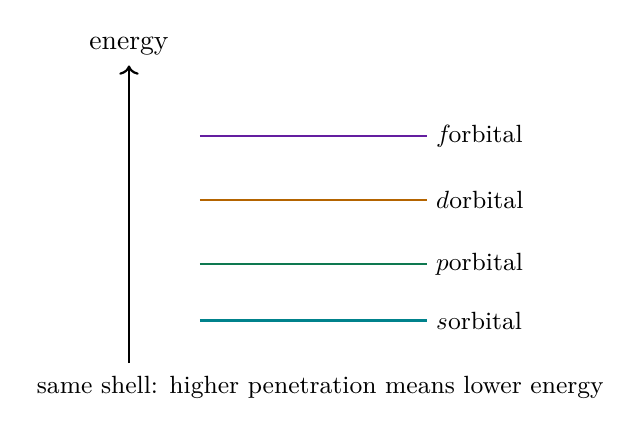
\begin{tikzpicture}[scale=0.9]
  \draw[->, thick] (0,0) -- (0,4.2) node[above] {energy};
  \foreach \y/\lab/\col in {0.6/$s$/myteal,1.4/$p$/mygreen,2.3/$d$/myamber,3.2/$f$/mypurple} {
    \draw[thick,\col] (1,\y) -- (4.2,\y);
    \node[right,font=\small] at (4.2,\y) {\lab orbital};
  }
  \node[font=\small, align=center] at (2.7,-0.35) {same shell: higher penetration means lower energy};
\end{tikzpicture}
\end{tcolorbox}

\subsection{Atomic Size, Ionization Energy, Electron Affinity and Electronegativity}
Across a period, $Z_{\mathrm{eff}}$ increases, so atomic size decreases and ionization energy generally increases. Down a group, new shells are added, so atomic size increases and ionization energy decreases.

\begin{tabularx}{\linewidth}{|B{3.2cm}|Y|Y|}
\hline
\textbf{Property} & \textbf{Across period} & \textbf{Down group} \\
\hline
Atomic radius & Decreases & Increases \\
\hline
Ionization energy & Generally increases & Decreases \\
\hline
Electron affinity & Becomes more negative generally & Less negative generally \\
\hline
Electronegativity & Increases & Decreases \\
\hline
Metallic character & Decreases & Increases \\
\hline
\end{tabularx}

\subsection{Polarizability, Oxidation States and Coordination}
Polarizability increases with size and diffuse electron cloud. Oxidation state depends on valence electron configuration. Coordination number and geometry depend on metal ion size, ligand size, and electron count.

\begin{tabularx}{\linewidth}{|B{2.8cm}|Y|Y|}
\hline
\textbf{Coordination number} & \textbf{Common geometry} & \textbf{Example type} \\
\hline
2 & Linear & $\mathrm{[Ag(NH_3)_2]^+}$ \\
\hline
4 & Tetrahedral or square planar & $\mathrm{[Ni(CN)_4]^{2-}}$ \\
\hline
6 & Octahedral & $\mathrm{[Fe(CN)_6]^{3-}}$ \\
\hline
\end{tabularx}

\subsection{Hard and Soft Acids and Bases}
HSAB principle says hard acids prefer hard bases and soft acids prefer soft bases.

\begin{tcolorbox}[defbox]
\textbf{Hard species} are small, highly charged, and weakly polarizable. \textbf{Soft species} are larger, lower charged, and highly polarizable.
\end{tcolorbox}

\subsection{Molecular Geometries}
VSEPR theory predicts geometry from electron-pair repulsion around the central atom.

\begin{tcolorbox}[tikzbox, title={Common VSEPR Shapes}]
\centering
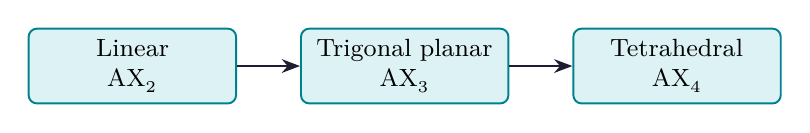
\begin{tikzpicture}[node distance=0.8cm and 0.8cm]
  \node[block] (lin) {Linear\\$\mathrm{AX_2}$};
  \node[block, right=of lin] (tri) {Trigonal planar\\$\mathrm{AX_3}$};
  \node[block, right=of tri] (tet) {Tetrahedral\\$\mathrm{AX_4}$};
  \draw[arrow] (lin) -- (tri);
  \draw[arrow] (tri) -- (tet);
\end{tikzpicture}
\end{tcolorbox}

\begin{tcolorbox}[exambox, title={Exam Points}]
\begin{itemize}[leftmargin=*, itemsep=2pt, topsep=2pt]
  \item Explain periodic trends using $Z_{\mathrm{eff}}$, shielding, and shell number.
  \item For orbital energy, mention penetration order $s>p>d>f$.
  \item HSAB questions need definition plus examples.
  \item Geometry questions should mention electron pairs before shape.
\end{itemize}
\end{tcolorbox}

% ===============================================================================
\section{Detailed Periodic Trend Analysis}
% ===============================================================================

\subsection{Shielding Order and Slater-Type Reasoning}
Shielding is not equal for all orbitals. Inner-shell electrons shield strongly, while electrons in the same shell shield only partially. Poor shielding by $d$ and $f$ electrons explains many irregular periodic trends.

\begin{tabularx}{\linewidth}{|B{3.2cm}|Y|Y|}
\hline
\textbf{Electron type} & \textbf{Shielding ability} & \textbf{Consequence} \\
\hline
$s$ electron & Strong penetration and good shielding & Feels high $Z_{\mathrm{eff}}$ \\
\hline
$p$ electron & Moderate shielding & Higher energy than same-shell $s$ \\
\hline
$d$ electron & Poor shielding & Causes transition-series contraction \\
\hline
$f$ electron & Very poor shielding & Causes lanthanide contraction \\
\hline
\end{tabularx}

\subsection{Successive Ionization Energies}
Successive ionization energies always increase because after removal of one electron, the remaining electrons are held more strongly by the positive ion.
\[
\mathrm{IE_1<IE_2<IE_3<\cdots}
\]
A sudden jump in ionization energy indicates removal of an electron from an inner shell.

\begin{tcolorbox}[examplebox, title={Solved Example: Identifying Valence Electrons}]
If successive ionization energies show the pattern:
\[
580,\quad 1820,\quad 2750,\quad 11600\ \mathrm{kJ\,mol^{-1}}
\]
the large jump occurs after the third electron. Therefore the atom has \textbf{three valence electrons}.
\end{tcolorbox}

\subsection{Diagonal Relationship}
Some second-period elements resemble third-period elements diagonally placed in the periodic table. Examples include Li--Mg, Be--Al, and B--Si. This occurs because size and charge density become comparable.

\begin{tabularx}{\linewidth}{|B{3cm}|Y|Y|}
\hline
\textbf{Pair} & \textbf{Common similarities} & \textbf{Reason} \\
\hline
Li and Mg & Form nitrides; carbonates decompose on heating & Similar charge density \\
\hline
Be and Al & Amphoteric oxides and covalent halides & Small size and high polarizing power \\
\hline
B and Si & Covalent compounds and acidic oxides & Similar electronegativity trend \\
\hline
\end{tabularx}

\subsection{Oxidation States and Inert Pair Effect}
For heavier $p$-block elements, the outer $ns^2$ electron pair becomes less available for bonding. This is called inert pair effect. It stabilizes lower oxidation states.

\begin{tcolorbox}[defbox]
\textbf{Inert pair effect:} Reluctance of the outermost $ns^2$ electron pair of heavier elements to participate in bonding.
\end{tcolorbox}

\begin{tabularx}{\linewidth}{|B{3cm}|Y|Y|}
\hline
\textbf{Group} & \textbf{Higher oxidation state} & \textbf{Lower oxidation state stabilized down group} \\
\hline
Group 13 & $+3$ & $+1$ in Tl \\
\hline
Group 14 & $+4$ & $+2$ in Pb \\
\hline
Group 15 & $+5$ & $+3$ in Bi \\
\hline
\end{tabularx}

\subsection{HSAB Applications}
HSAB theory predicts stability of complexes and salts. Hard-hard and soft-soft combinations are more stable than hard-soft combinations.

\begin{tabularx}{\linewidth}{|B{3.0cm}|Y|Y|}
\hline
\textbf{Acid / base type} & \textbf{Examples} & \textbf{Preferred partner} \\
\hline
Hard acids & $\mathrm{H^+, Li^+, Al^{3+}, Fe^{3+}}$ & Hard bases \\
\hline
Soft acids & $\mathrm{Ag^+, Hg^{2+}, Pt^{2+}}$ & Soft bases \\
\hline
Hard bases & $\mathrm{F^-, OH^-, H_2O, NH_3}$ & Hard acids \\
\hline
Soft bases & $\mathrm{I^-, S^{2-}, CO, PR_3}$ & Soft acids \\
\hline
\end{tabularx}

\begin{tcolorbox}[examplebox, title={Solved Example: HSAB Prediction}]
$\mathrm{Ag^+}$ is a soft acid. Between $\mathrm{F^-}$ and $\mathrm{I^-}$, iodide is softer. Therefore $\mathrm{AgI}$ is more stable and less soluble than expected from simple charge arguments.
\end{tcolorbox}

\subsection{VSEPR Shapes and Lone Pair Effect}
Lone pairs repel more strongly than bond pairs. The repulsion order is:
\[
\text{lone pair-lone pair}>\text{lone pair-bond pair}>\text{bond pair-bond pair}
\]

\begin{tabularx}{\linewidth}{|B{2.8cm}|Y|Y|}
\hline
\textbf{Molecule type} & \textbf{Shape} & \textbf{Example} \\
\hline
$\mathrm{AX_2}$ & Linear & $\mathrm{BeCl_2}$, $\mathrm{CO_2}$ \\
\hline
$\mathrm{AX_3}$ & Trigonal planar & $\mathrm{BF_3}$ \\
\hline
$\mathrm{AX_3E}$ & Trigonal pyramidal & $\mathrm{NH_3}$ \\
\hline
$\mathrm{AX_2E_2}$ & Bent & $\mathrm{H_2O}$ \\
\hline
$\mathrm{AX_4}$ & Tetrahedral & $\mathrm{CH_4}$ \\
\hline
\end{tabularx}

\begin{tcolorbox}[masonbox, title={Periodic Properties: 10-Mark Answer Framework}]
\begin{enumerate}[leftmargin=*, itemsep=3pt, topsep=2pt]
  \item Define the property.
  \item State the trend across period and down group.
  \item Explain trend using $Z_{\mathrm{eff}}$, shielding, and shell size.
  \item Mention exceptions if relevant.
  \item Add one example or application such as HSAB or VSEPR shape.
\end{enumerate}
\end{tcolorbox}

\subsection{Atomic and Ionic Radius: Detailed Trend}
Atomic radius decreases across a period because effective nuclear charge increases while electrons enter the same shell. Down a group, radius increases because a new shell is added.

\begin{tabularx}{\linewidth}{|B{3.2cm}|Y|Y|}
\hline
\textbf{Species compared} & \textbf{Trend} & \textbf{Reason} \\
\hline
Cations vs atoms & Cations are smaller & Electron loss reduces repulsion and may remove outer shell \\
\hline
Anions vs atoms & Anions are larger & Extra electron increases electron-electron repulsion \\
\hline
Isoelectronic species & Radius decreases with increasing nuclear charge & Same electrons pulled by larger $Z$ \\
\hline
\end{tabularx}

\begin{tcolorbox}[examplebox, title={Solved Example: Isoelectronic Radius Order}]
$\mathrm{N^{3-}}$, $\mathrm{O^{2-}}$, $\mathrm{F^-}$, $\mathrm{Na^+}$ and $\mathrm{Mg^{2+}}$ are isoelectronic with 10 electrons.

Higher nuclear charge pulls the same electron cloud more strongly:
\[
\mathrm{N^{3-}>O^{2-}>F^->Na^+>Mg^{2+}}
\]
\end{tcolorbox}

\subsection{Electron Affinity and Exceptions}
Electron affinity generally becomes more negative across a period, but exceptions occur due to stable half-filled or filled configurations and small size.

\begin{tabularx}{\linewidth}{|B{3.2cm}|Y|Y|}
\hline
\textbf{Exception} & \textbf{Observation} & \textbf{Reason} \\
\hline
N less negative than C/O & N resists electron gain & Stable half-filled $2p^3$ configuration \\
\hline
F less negative than Cl & Cl has more negative electron affinity & Very small F atom has high electron-electron repulsion \\
\hline
Noble gases & Positive or very low tendency & Stable closed shell \\
\hline
\end{tabularx}

\subsection{Electronegativity Scales}
Electronegativity is not directly measured; it is assigned using scales. The Pauling scale is most common in basic chemistry.

\begin{tabularx}{\linewidth}{|B{3cm}|Y|Y|}
\hline
\textbf{Scale} & \textbf{Basis} & \textbf{Use} \\
\hline
Pauling & Bond energy differences & Most common qualitative scale \\
\hline
Mulliken & Average of ionization energy and electron affinity & Connects to atomic properties \\
\hline
Allred-Rochow & Electrostatic attraction by nucleus & Uses effective nuclear charge and radius \\
\hline
\end{tabularx}

\subsection{Polarization and Fajan's Rules}
Fajan's rules explain covalent character in ionic compounds. A small highly charged cation polarizes a large anion strongly, increasing covalent character.

\begin{tcolorbox}[masonbox, title={Fajan's Rules}]
\begin{itemize}[leftmargin=*, itemsep=2pt, topsep=2pt]
  \item Smaller cation has greater polarizing power.
  \item Higher cation charge has greater polarizing power.
  \item Larger anion is more easily polarized.
  \item Cations with pseudo-noble gas configuration polarize more strongly.
\end{itemize}
\end{tcolorbox}

\begin{tcolorbox}[examplebox, title={Solved Example: Covalent Character}]
$\mathrm{AlCl_3}$ has more covalent character than $\mathrm{NaCl}$ because $\mathrm{Al^{3+}}$ is smaller and more highly charged than $\mathrm{Na^+}$, so it polarizes $\mathrm{Cl^-}$ more strongly.
\end{tcolorbox}

\subsection{Coordination Number and Geometry in Complexes}
Coordination number is the number of ligand donor atoms directly attached to the metal ion. Geometry depends on coordination number and electronic arrangement.

\begin{tabularx}{\linewidth}{|B{2.8cm}|Y|Y|}
\hline
\textbf{Coordination number} & \textbf{Geometry} & \textbf{Typical comment} \\
\hline
2 & Linear & Common for $\mathrm{Ag^+}$ and $\mathrm{Cu^+}$ complexes \\
\hline
4 & Tetrahedral & Common when ligands are bulky or weak-field \\
\hline
4 & Square planar & Common for $d^8$ metal ions like $\mathrm{Pt^{2+}}$ \\
\hline
6 & Octahedral & Most common geometry for transition-metal complexes \\
\hline
\end{tabularx}

\begin{tcolorbox}[masonbox, title={Previous-Year Style Questions}]
\begin{enumerate}[leftmargin=*, itemsep=4pt, topsep=2pt]
  \item Explain effective nuclear charge and shielding with periodic trends.
  \item Discuss trends in atomic radius, ionization energy and electronegativity.
  \item Explain penetration of $s$, $p$, $d$, $f$ orbitals and its effect on energy.
  \item State HSAB principle and predict stable acid-base combinations.
  \item Explain VSEPR shapes and coordination geometries with examples.
\end{enumerate}
\end{tcolorbox}

\subsection{Common Exceptions and Exam Traps}
Periodic trends are general rules, but exam questions often test exceptions. Mentioning the reason behind exceptions improves answer quality.

\begin{tabularx}{\linewidth}{|B{3.2cm}|Y|Y|}
\hline
\textbf{Trend exception} & \textbf{Observation} & \textbf{Reason} \\
\hline
Be and B ionization energy & $\mathrm{IE(Be)>IE(B)}$ & Electron removed from B enters higher-energy $2p$ orbital \\
\hline
N and O ionization energy & $\mathrm{IE(N)>IE(O)}$ & N has stable half-filled $2p^3$ arrangement \\
\hline
Ga smaller than Al anomaly & Size does not increase as expected & Poor shielding by filled $3d$ electrons \\
\hline
Lanthanide contraction & Similar radii of 4d and 5d elements & Poor shielding by $4f$ electrons \\
\hline
\end{tabularx}

\begin{tcolorbox}[examplebox, title={Exam Answer: Why \texorpdfstring{$\mathrm{IE(N)>IE(O)}$}{IE(N)>IE(O)}?}]
Nitrogen has electronic configuration $1s^2 2s^2 2p^3$, where the three $p$ electrons are half-filled and relatively stable. Oxygen has $1s^2 2s^2 2p^4$, so one $p$ orbital contains paired electrons. Removing one electron from oxygen reduces electron-electron repulsion, so oxygen has lower first ionization energy than nitrogen.
\end{tcolorbox}
\newpage
\begin{center}
  {\large\bfseries\color{myred} Quick Revision --- Module 5}\\[3pt]
  {\small\color{mydark} Periodic Properties $|$ BS-CH101}
\end{center}
\noindent{\color{myred}\rule{\linewidth}{1.2pt}}
\vspace{4pt}

\begin{tcolorbox}[formulabox, title={Key Formulas at a Glance}]
\begin{tabularx}{\linewidth}{|B{4.0cm}|Y|}
\hline
\textbf{Formula / Rule} & \textbf{Meaning} \\
\hline
$Z_{\mathrm{eff}}=Z-\sigma$ & Effective nuclear charge felt by valence electron. \\
\hline
$s>p>d>f$ & Penetration order within a shell. \\
\hline
$E(ns)<E(np)<E(nd)<E(nf)$ & Orbital energy order for same principal shell in multi-electron atoms. \\
\hline
$\mathrm{IE_1}<\mathrm{IE_2}<\mathrm{IE_3}$ & Successive ionization energies increase. \\
\hline
$\mu=\alpha E$ & Induced dipole moment relation; $\alpha$ is polarizability. \\
\hline
\end{tabularx}
\end{tcolorbox}

\begin{tcolorbox}[defbox, title={One-Line Definitions}]
\begin{itemize}[leftmargin=*, itemsep=2pt, topsep=2pt]
  \item \textbf{Effective nuclear charge:} Net positive charge experienced by an electron.
  \item \textbf{Shielding:} Reduction of nuclear attraction due to inner electrons.
  \item \textbf{Penetration:} Ability of an orbital to approach the nucleus.
  \item \textbf{Ionization energy:} Energy required to remove an electron from gaseous atom.
  \item \textbf{Electron affinity:} Energy change when an electron is added to gaseous atom.
  \item \textbf{Electronegativity:} Tendency of atom to attract bonded electron pair.
  \item \textbf{HSAB principle:} Hard acids bind hard bases and soft acids bind soft bases.
\end{itemize}
\end{tcolorbox}

\begin{tcolorbox}[exambox, title={Frequently Asked / Viva Questions}]
\begin{enumerate}[topsep=0pt, label=\textbf{Q\arabic*.}, itemsep=5pt]
  \item \Q{Define effective nuclear charge.}
    It is the net nuclear charge felt by an electron after shielding.
  \item \Q{Why does atomic radius decrease across a period?}
    $Z_{\mathrm{eff}}$ increases and pulls electrons closer.
  \item \Q{Why does ionization energy decrease down a group?}
    Atomic size and shielding increase, so valence electrons are removed more easily.
  \item \Q{Write the penetration order.}
    $s>p>d>f$.
  \item \Q{Why is an $s$ orbital lower in energy than a $p$ orbital of same shell?}
    The $s$ orbital penetrates closer to the nucleus and feels greater $Z_{\mathrm{eff}}$.
  \item \Q{What is polarizability?}
    Ease with which an electron cloud is distorted by an electric field.
  \item \Q{What is HSAB principle?}
    Hard acids prefer hard bases and soft acids prefer soft bases.
  \item \Q{Give examples of hard and soft bases.}
    Hard bases: $\mathrm{F^-}$, $\mathrm{OH^-}$; soft bases: $\mathrm{I^-}$, $\mathrm{S^{2-}}$.
  \item \Q{What decides coordination geometry?}
    Coordination number, ligand field, metal ion size, and electron configuration.
  \item \Q{What is VSEPR theory used for?}
    It predicts molecular geometry from repulsion among electron pairs.
\end{enumerate}
\end{tcolorbox}

\begin{tcolorbox}[tikzbox, title={Summary Reference Table}]
\begin{tabularx}{\linewidth}{|B{3cm}|Y|Y|}
\hline
\textbf{Trend} & \textbf{Reason} & \textbf{Result} \\
\hline
Across period & $Z_{\mathrm{eff}}$ increases & Size decreases, IE increases \\
\hline
Down group & Shell number increases & Size increases, IE decreases \\
\hline
Penetration & $s$ enters closest to nucleus & $s$ orbital has lower energy \\
\hline
HSAB & Charge density and polarizability & Predicts stable acid-base pairs \\
\hline
\end{tabularx}
\end{tcolorbox}

\end{document}
